\subsection{Dalvik Executable File Format} \label{subsection:android-dex}
As explained in subsection~\ref{subsection:foundation-android-package}, an Android application is distributed using \gls{apk}s.
The \gls{apk} contains the Dalvik executable file \textit{classes.dex}.
Figure~\ref{fig:dex} shows the structure of this file.
First, the actual bytecode marked red in figure~\ref{fig:dex} is explained, then the checksum and signature mechanism.
\newline
\begin{figure}[h]
    \centering
    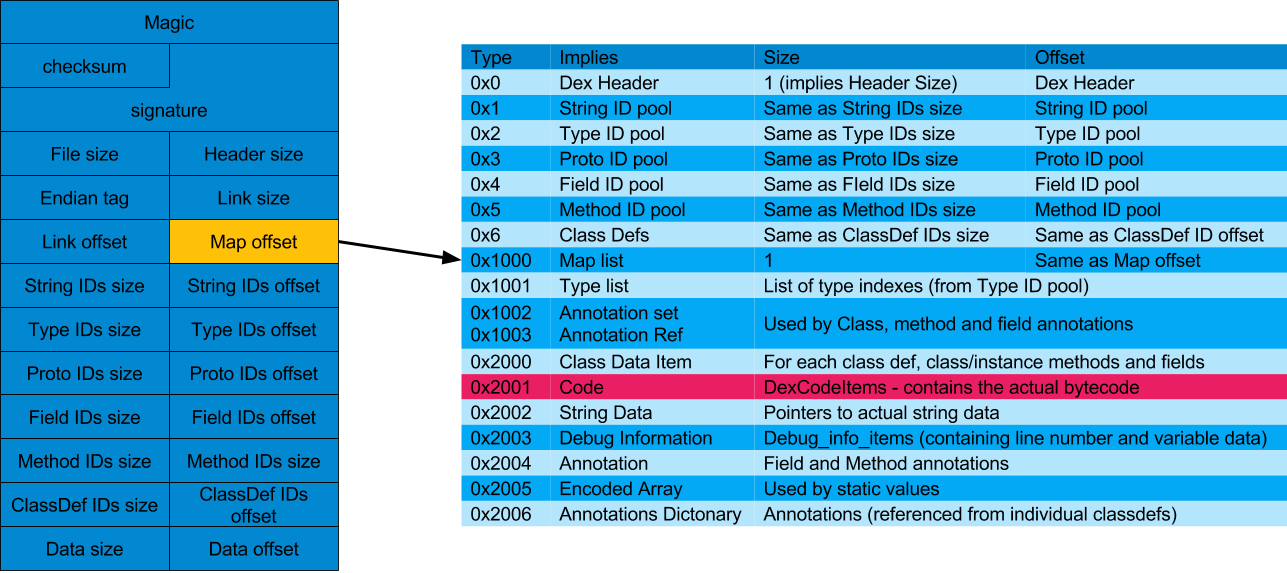
\includegraphics[width=1\textwidth]{data/dex.png}
    \caption{\gls{dex} file format \cite{andevconDalvikART}}
    \label{fig:dex}
\end{figure}
The bytecode is a sequence of instructions consisting of an opcode and a number of arguments.
The opcode is 8 bit length and determines number and interpretation, e.g. boolean, constant or variable, of its arguments.
Instructions are of variable length and aligned to multiples of 16 bit.
Instead of using actual data as arguments, references to Dalvik registers are used. \cite{androidDalvik} \cite{opcodes}
\newline
In the context of this work, the most important parts of the header are the checksum and the signature.
The checksum field contains the Adler32 checksum of the \gls{dex} file.
It is calculated from all fields of the file except the magic field and itself.
The checksum is used to detect whether the file is corrupt.
The signature field contains the SHA-1 hash value of the file minus the magic field, checksum field and itself.
The file can be uniquely identified by the signature, which is also part of the code signing stored in the manifest files to ensure integrity and authenticity.
When the \gls{dex} file is modified, both the checksum and signature have to be recalculated and updated. \cite{developersDalvik} \cite{ehringerDalvik}
\newline
Dex bytecode can be optimized.
Upon installation, improvements specific to the underlying architecture can be applied to the bytecode.
The resulting \gls{dex} file is called \gls{odex}.
The optimization is executed by a program called \textit{dexopt} which is part of the Android platform.
The semantics of the two files is the same, but the \gls{odex} file has the better performance.
\newline
Like Java bytecode, Dalvik bytecode can be reverse engineered back to Java source code.
As it contains a lot of meta information, e.g. variable and method names, the resulting Java code is reasonably easy to understand, exposing the application logic.
